\documentclass[master=eelt,masteroption=ei]{kulemt}
\setup{% Remove the "%" on the next line when using UTF-8 character encoding
  inputenc=utf8,
  title={The best master's thesis ever},
  author={First Author\and Second Author},
  promotor={Prof.\,dr.\,ir.\ Knows Better},
  assessor={Ir.\,Kn. Owsmuch\and K. Nowsrest},
  assistant={Ir.\ An~Assistent \and A.~Friend}}
% Remove the "%" on the next line for generating the cover page
%\setup{coverpageonly}
% Remove the "%" before the next "\setup" to generate only the first pages
% (e.g., if you are a Word user).
%\setup{frontpagesonly}

% Choose the main text font (e.g., Latin Modern)
\setup{font=lm}

% If you want to include other LaTeX packages, do it here. 

% Finally the hyperref package is used for pdf files.
% This can be commented out for printed versions.
\usepackage[pdfusetitle,colorlinks,plainpages=false]{hyperref}

%%%%%%%
% The lipsum package is used to generate random text.
% You never need this in a real master's thesis text!
\IfFileExists{lipsum.sty}%
 {\usepackage{lipsum}\setlipsumdefault{11-13}}%
 {\newcommand{\lipsum}[1][11-13]{\par And some text: lipsum ##1.\par}}
%%%%%%%

%\includeonly{chap-n}
\begin{document}

\begin{preface}
  I would like to thank everybody who kept me busy the last year,
  especially my promoter and my assistants. I would also like to thank the
  jury for reading the text. My sincere gratitude also goes to my wive and
  the rest of my family.
\end{preface}

\tableofcontents*

\begin{abstract}
  The \texttt{abstract} environment contains a more extensive overview of
  the work. But it should be limited to one page.

  \lipsum[1]
\end{abstract}

% A list of figures and tables is optional
%\listoffigures
%\listoftables
% If you only have a few figures and tables you can use the following instead
\listoffiguresandtables
% The list of symbols is also optional.
% This list must be created manually, e.g., as follows:
\chapter{List of Abbreviations and Symbols}
\section*{Abbreviations}
\begin{flushleft}
  \renewcommand{\arraystretch}{1.1}
  \begin{tabularx}{\textwidth}{@{}p{12mm}X@{}}
    LoG   & Laplacian-of-Gaussian \\
    MSE   & Mean Square error \\
    PSNR  & Peak Signal-to-Noise ratio \\
  \end{tabularx}
\end{flushleft}
\section*{Symbols}
\begin{flushleft}
  \renewcommand{\arraystretch}{1.1}
  \begin{tabularx}{\textwidth}{@{}p{12mm}X@{}}
    42    & ``The Answer to the Ultimate Question of Life, the Universe,
            and Everything'' according to \cite{h2g2} \\
    $c$   & Speed of light \\
    $E$   & Energy \\
    $m$   & Mass \\
    $\pi$ & The number pi \\
  \end{tabularx}
\end{flushleft}

% Now comes the main text
\mainmatter

\chapter{Introduction}
\label{cha:intro}
For many years computer programs have been plagued by vulnerabilities that can be exploited in order to gain control over the execution of a program.
Several classes of these vulnerabilities arise from bugs in the source code and are related to low level control over memory.
Spatial memory issues are vulnerabilities that arise from accessing memory that is outside of the bounds that are supposed to be accessed.
Temporal memory issues on the other hand arise from accessing memory after the reference to that memory is supposed to have been invalidated.
Some famous examples of spatial and temporal memory issues are buffer overflows and use after free whereby an attacker can write to memory that is not supposed to be written to\tomi{add some references whenever you make claims like this; you have very few references atm}.

Over the past decades, several solutions to these issues have been presented and implemented.
One of the most popular solution is the usage of memory safe programming languages that deny the programmer low level access to the memory\tomi{some example refs}.
Instead, the memory is managed by a language runtime and deallocated by a garbage collector.
This solution, however, has a significant performance impact and is thus not applicable to performance sensitive programs such as kernels, browsers and low level system libraries.
These types of programs remain vulnerable and are often a vector for malware to gain control over a system.
A class of devices that are especially vulnerable to these issues are embedded devices, since they have constrained resources and programmers require low level memory management features to gain reasonable performance.
With the advent of the Internet of Things (IoT), these embedded devices are expected to increase in number dramatically\tomi{ref}.

Over the past few years programming languages with strong type systems have gained renewed attention as a way to mitigate these issues and improve security\tomi{strong claim; prove with ref or weaken}.
One of the most popular of these is the Rust programming language\tomi{ref}.
Rust offers a number of security features, but in this thesis we will focus on Rust's ownership and borrowing system.
This system limits what a programmer can do with references to an object in memory, ensuring that memory is always accessed in a safe manner, and statically guaranteeing thread safety.
One of the most important principles of this system is the principle of ``aliasing XOR mutability'' which means that references to a resource in memory are either allowed to mutate the resource or are read-only and can be copied, but not both.
This prevents concurrent write accesses and concurrent read and write access to a resource in memory, which ensures the absence of things like data races.

However, when a Rust program is compiled, it is usually converted into an unsafe assembly language that does not have any of these safety guarantees\tomi{refer to some secure compilation paper}.
This might, for example, open the programs up to attacks on the assembly level if they are linked with libraries that are not written in a programming language with the same safety guarantees.
In this thesis we explore an extension to the capability machine architecture CHERI in order to provide support on the assembly level for the safety guarantees that the Rust programming language offers.

Hardware capabilities are unforgeable pointers that represent authority over a region of memory.
They are comparable to software fat pointers in that they enforce bounds checking and hold permissions that specify how a region of memory can be used.
This model is very effective at combating spatial memory issues, but is less suited to enforce the temporal memory safety guarantees offered by languages with strong type systems.
Nevertheless, CHERI does offer some hardware primitives that software can build upon to strengthen their defense against temporal memory issues.
In this thesis we will add a new type of capability called \textit{borrowed capability}.
This new type of capability is designed to mimic Rust's ownership and borrowing system, but it could be seen in a wider context as an addition to the types of revocation that are already offered by CHERI.

In summary, the goal of this thesis is to design an extension to the CHERI architecture that offers the same memory and thread safety guarantees as the Rust programming language.
\tomi{Mention section numbers in explanation below, since you're going over the sections anyways + update to include discussion section}
To test our design, we will implement it in the Sail specification language, extend the LLVM project to create an assembler for our extension and run test programs on the emulator generated by Sail.
We start off by giving background information about Rust and CHERI as well as information about RISC-V and the Sail language which will be essential for the implementation of our design.
Next, we provide an overview of our design, followed by the details of its implementation in Sail and the details of the LLVM extension.
Finally, we will evaluate our design by constructing a number of assembly example programs and reason about how well they mimic the Rust ownership and borrowing system.

%%% Local Variables: 
%%% mode: latex
%%% TeX-master: "thesis"
%%% End: 

\chapter{The First Chapter}
\label{cha:1}
A chapter is a logical unit. It normally starts with an introduction, which
you are reading now. The last topic of the chapter holds the conclusion.

\section{The First Topic of the Chapter}
First comes the introduction to this topic.

\lipsum[55]

\subsection{An item}
Please don't abuse enumerations: short enumerations shouldn't use
``\verb|itemize|'' or ``\texttt{enumerate}'' environments.
So \emph{never write}: 
\begin{quote}
  The Eiffel tower has three floors:
  \begin{itemize}
  \item the first one;
  \item the second one;
  \item the third one.
  \end{itemize}
\end{quote}
But write:
\begin{quote}
  The Eiffel tower has three floors: the first one, the second one, and the
  third one.
\end{quote}

\section{A Second Topic}
\lipsum[64]

\subsection{Another item}
\lipsum[56-57]

\section{Conclusion}
The final section of the chapter gives an overview of the important results
of this chapter. This implies that the introductory chapter and the
concluding chapter don't need a conclusion.

\lipsum[66]

%%% Local Variables: 
%%% mode: latex
%%% TeX-master: "thesis"
%%% End: 

\chapter{The Next Chapter}
\label{cha:2}
\lipsum[77]

\section{The First Topic of this Chapter}
\lipsum[78]

\subsection{An item}
A master's thesis is never an isolated work. This means that your text must
contain references. On-line documents\cite{wiki} as well as
books\cite{pratchett06:_good_omens} can be referenced.

\section{Figures}
Figures are used to add illustrations to the text. The \fref{fig:logo} shows
the KU~Leuven logo as an illustration.
\begin{figure}
  \centering
  \includegraphics{logokul}
  \caption{The KU~Leuven logo.}
  \label{fig:logo}
\end{figure}

\section{Tables}
Tables are used to present data neatly arranged. A table is normally
not a spreadsheet! Compare \tref{tab:wrong} en \tref{tab:ok}: which table do
you prefer?

\begin{table}
  \centering
  \begin{tabular}{||l|lr||} \hline
    gnats     & gram      & \$13.65 \\ \cline{2-3}
              & each      & .01 \\ \hline
    gnu       & stuffed   & 92.50 \\ \cline{1-1} \cline{3-3}
    emu       &           & 33.33 \\ \hline
    armadillo & frozen    & 8.99 \\ \hline
  \end{tabular}
  \caption{A table with the wrong layout.}
  \label{tab:wrong}
\end{table}

\begin{table}
  \centering
  \begin{tabular}{@{}llr@{}} \toprule
    \multicolumn{2}{c}{Item} \\ \cmidrule(r){1-2}
    Animal    & Description & Price (\$)\\ \midrule
    Gnat      & per gram    & 13.65 \\
              & each        & 0.01 \\
    Gnu       & stuffed     & 92.50 \\
    Emu       & stuffed     & 33.33 \\
    Armadillo & frozen      & 8.99 \\ \bottomrule
  \end{tabular}
  \caption{A table with the correct layout.}
  \label{tab:ok}
\end{table}

\section{Lorem Ipsum}
This section is added to check headers and footers. So this chapter must at
least contain three pages. To make sure that we get the required amount,
the \textsf{lipsum} package isn't used but the text is put directly in the
text.

\subsection{Lorem ipsum dolor sit amet, consectetur adipiscing elit}
Sed nec tortor id felis tristique sodales. Nulla nec massa eu dui fermentum
tincidunt. Integer ullamcorper ante eget eros posuere faucibus. Nam id
ligula ut augue pulvinar vulputate id at purus. Aenean condimentum tortor
eu mi placerat eget eleifend massa mollis. Nam est mi, sagittis quis
euismod eget, sagittis in nibh. Proin elit turpis, aliquam et imperdiet
sed, volutpat eu turpis.

Pellentesque vel enim tellus, vitae egestas turpis. Praesent malesuada elit
non nisi sollicitudin non blandit lacus tincidunt. Morbi blandit urna at
lectus ornare laoreet. Suspendisse turpis diam, lobortis dictum luctus
quis, commodo at lorem. Integer lacinia convallis ultricies. Sed quis augue
neque, eu malesuada arcu. Nullam vehicula, purus vitae sagittis pulvinar,
erat eros semper massa, eu egestas nibh erat quis magna. Cras pellentesque,
nisl eu dapibus volutpat, urna augue ornare quam, quis egestas lectus nulla
a lectus.

Vivamus dictum libero in massa cursus sed vulputate eros imperdiet. Donec
lacinia, libero ac lobortis egestas, nibh dui ornare arcu, luctus porttitor
velit massa sit amet quam. Maecenas scelerisque laoreet diam, vitae congue
quam adipiscing vitae. Aliquam cursus nisl a leo convallis eleifend
fermentum massa porta. Nunc libero quam, dapibus dapibus molestie sit amet,
faucibus vel nunc.

\subsection{Praesent auctor venenatis posuere}
Sed tellus augue, molestie in pulvinar lacinia, dapibus non ipsum. Fusce
vitae mi vitae enim ullamcorper hendrerit eu malesuada est. Proin iaculis
ante sed nibh tincidunt vel interdum libero posuere. Vivamus accumsan metus
quis felis congue suscipit dapibus enim mattis. Fusce mattis tortor eget
ipsum interdum sagittis auctor id metus.

Integer diam lacus, pharetra sit amet tempor et, tristique non lorem.
Aenean auctor, nisi eu interdum fermentum, lectus massa adipiscing elit,
sed facilisis orci odio a lectus. Proin mi nibh, tempus quis porta a,
viverra quis enim. In sollicitudin egestas libero, quis viverra velit
molestie eget. Nulla rhoncus, dolor a mollis vestibulum, lacus elit semper
nisi, nec sollicitudin sem urna eu magna. Nunc sed est urna, euismod congue
mi.

\subsection{Cras vulputate ultricies venenatis}
Vivamus eros urna, sodales accumsan semper vel, lobortis sit amet mauris.
Etiam condimentum eleifend lorem, ullamcorper ornare lectus aliquet vitae.
Praesent massa enim, interdum sit amet semper et, venenatis ut elit.
Quisque faucibus, quam ac lacinia imperdiet, nulla neque elementum purus,
tempus rutrum justo massa porta sapien. Vestibulum ante ipsum primis in
faucibus orci luctus et ultrices posuere cubilia Curae; Sed ultrices
interdum mi, et rhoncus sapien rutrum sed.

Duis elit orci, molestie quis sollicitudin sed, convallis non ante.
Maecenas tincidunt condimentum justo, et ultricies leo tristique vitae.
Vestibulum quis quam non lectus dapibus eleifend a vitae nibh. Nam nibh
justo, pharetra quis iaculis consequat, elementum quis justo. Etiam mollis
lacinia lacus, nec sollicitudin urna lobortis ac. Nulla facilisi.

Proin placerat risus eleifend erat ultricies placerat. Etiam rutrum magna
nec turpis euismod consectetur. Phasellus tortor odio, lacinia imperdiet
condimentum sed, faucibus commodo erat. Phasellus sed felis id ante
placerat ultrices. Aenean tempor justo in tortor volutpat eu auctor dolor
mollis. Aenean sit amet risus urna. Morbi viverra vehicula cursus.

\subsection{Donec nibh ante, consectetur et posuere id, tempus nec arcu}
Curabitur a tellus aliquet ipsum pellentesque scelerisque. Etiam congue,
risus et volutpat rutrum, est purus dapibus leo, non cursus metus felis
eget ligula. Vivamus facilisis tristique turpis, ut pretium lectus luctus
eleifend. Fusce magna sapien, ullamcorper vitae fringilla id, euismod quis
ante.

Phasellus volutpat, nunc et pharetra semper, sem justo adipiscing mauris,
id blandit magna quam et orci. Vestibulum a erat purus, ut molestie ante.
Vestibulum ante ipsum primis in faucibus orci luctus et ultrices posuere
cubilia Curae; Proin turpis diam, consequat ut ullamcorper ut, consequat eu
orci. Sed metus risus, fringilla nec interdum vel, interdum eu nunc.
Suspendisse vel sapien orci.

\subsection{Morbi et mauris tempus purus ornare vehicula}
Mauris sit amet diam quam, eget luctus purus. Sed faucibus, risus semper
eleifend iaculis, mi turpis bibendum nisl, quis cursus nibh nisl sit amet
ipsum. Vestibulum tempor urna vitae mi auctor malesuada eget non ligula.
Nullam convallis, diam vel ultrices auctor, eros eros egestas elit, sed
accumsan arcu tortor eget leo. Vestibulum orci purus, porttitor in pharetra
eget, tincidunt eget nisl. Nullam sit amet nulla dui, facilisis vestibulum
dui.

Donec faucibus facilisis mauris ac cursus. Duis rhoncus quam sed nisi
laoreet eu scelerisque massa tincidunt. Vivamus sit amet libero nec arcu
imperdiet tempor quis non libero. Sed consequat dignissim justo. Phasellus
ullamcorper, velit quis posuere vulputate, felis erat tincidunt mauris, at
vestibulum justo lectus et turpis. Maecenas lacinia convallis euismod.
Quisque egestas fermentum sapien eu dictum. Sed nec lacus in purus dictum
consequat quis vel nisl. Fusce non urna sem. Curabitur eu diam vitae elit
accumsan blandit. Nullam fermentum nunc et leo dictum laoreet. Donec semper
varius velit vel fringilla. Vivamus eu orci nunc.

\section{Conclusion}
The final section of the chapter gives an overview of the important results
of this chapter. This implies that the introductory chapter and the
concluding chapter don't need a conclusion.

\lipsum[66]

%%% Local Variables: 
%%% mode: latex
%%% TeX-master: "thesis"
%%% End: 

% ... and so on until
\chapter{The Final Chapter}
\label{cha:n}
\lipsum[79]

\section{The First Topic of this Chapter}
\subsection{Item 1}
\subsubsection{Sub-item 1}
\lipsum[80]

\subsubsection{Sub-item 2}
\lipsum[81]

\subsection{Item 2}
\lipsum[82]

\section{The Second Topic}
\lipsum[83-85]

\section{Conclusion}
\lipsum[86-88]

%%% Local Variables: 
%%% mode: latex
%%% TeX-master: "thesis"
%%% End: 

\chapter{Conclusion}
\label{cha:conclusion}
In this thesis we presented \textit{borrowed capabilities}, a new type of capability for CHERI that is designed to mirror the semantics of the Rust programming language.
We introduced the design for borrowed capabilities, revolving around binding capabilities to lifetime tokens and making these bound capabilities only dereferenceable when that lifetime token is present.
The design provides support for the ``aliasing XOR mutation'' principle by locking away capabilities in a borrow table and having both mutable and immutable borrow operations.
Concurrent use cases were taken into account by allowing lifetime tokens to split into multiple lifetime fractions that can be used by multiple threads at the same time.
We made a Sail implementation of both linear capabilities and borrowed capabilities and discussed the various design decisions relating to this implementation.
We extended the LLVM compiler project to be able to assemble programs using the instructions that were introduced in the design.
Finally we wrote sample assembly programs that mirror specific Rust programs to demonstrate how borrowed capabilities offer semantics that are similar to Rust's ownership and borrowing system and reasoned about the costs of the design of borrowed capbilities.
The assembly programs can be assembled by the LLVM assembler and run in the emulator that is produced by Sail.
From the assembly programs we can conclude that borrowed capabilities do indeed have semantics and guarantees that are similar to those that Rust provides.

There are some outstanding problems with borrowed capabilities that prevent them from being used as the target of a secure Rust compiler such as the behavior related to nested references.
Nevertheless, we think borrowed capabilities are a significant step towards supporting Rust's ownership and borrowing system at the assembly level.
While fitting the design of borrowed capabilities into CHERI is fairly simple and does not require expensive changes to CHERI, actually implementing borrowed capabilities in hardware could have significant extra costs.
The main limitations of borrowed capabilities such as lifetime id exhaustion may be mitigated or worked around.

We also considered borrowed capabilities as a new form of revocation in CHERI, supporting a model of mutual distrust between two parties.
While this thesis did not focus on the use of borrowed capabilities as a general form of revocation, we do think they are promising in this regard and this is an interesting direction to explore in future work.


%%% Local Variables: 
%%% mode: latex
%%% TeX-master: "thesis"
%%% End: 


% If you have appendices:
\appendixpage*          % if wanted
\appendix
\chapter{Sail Documentation}
\label{app:saildoc}
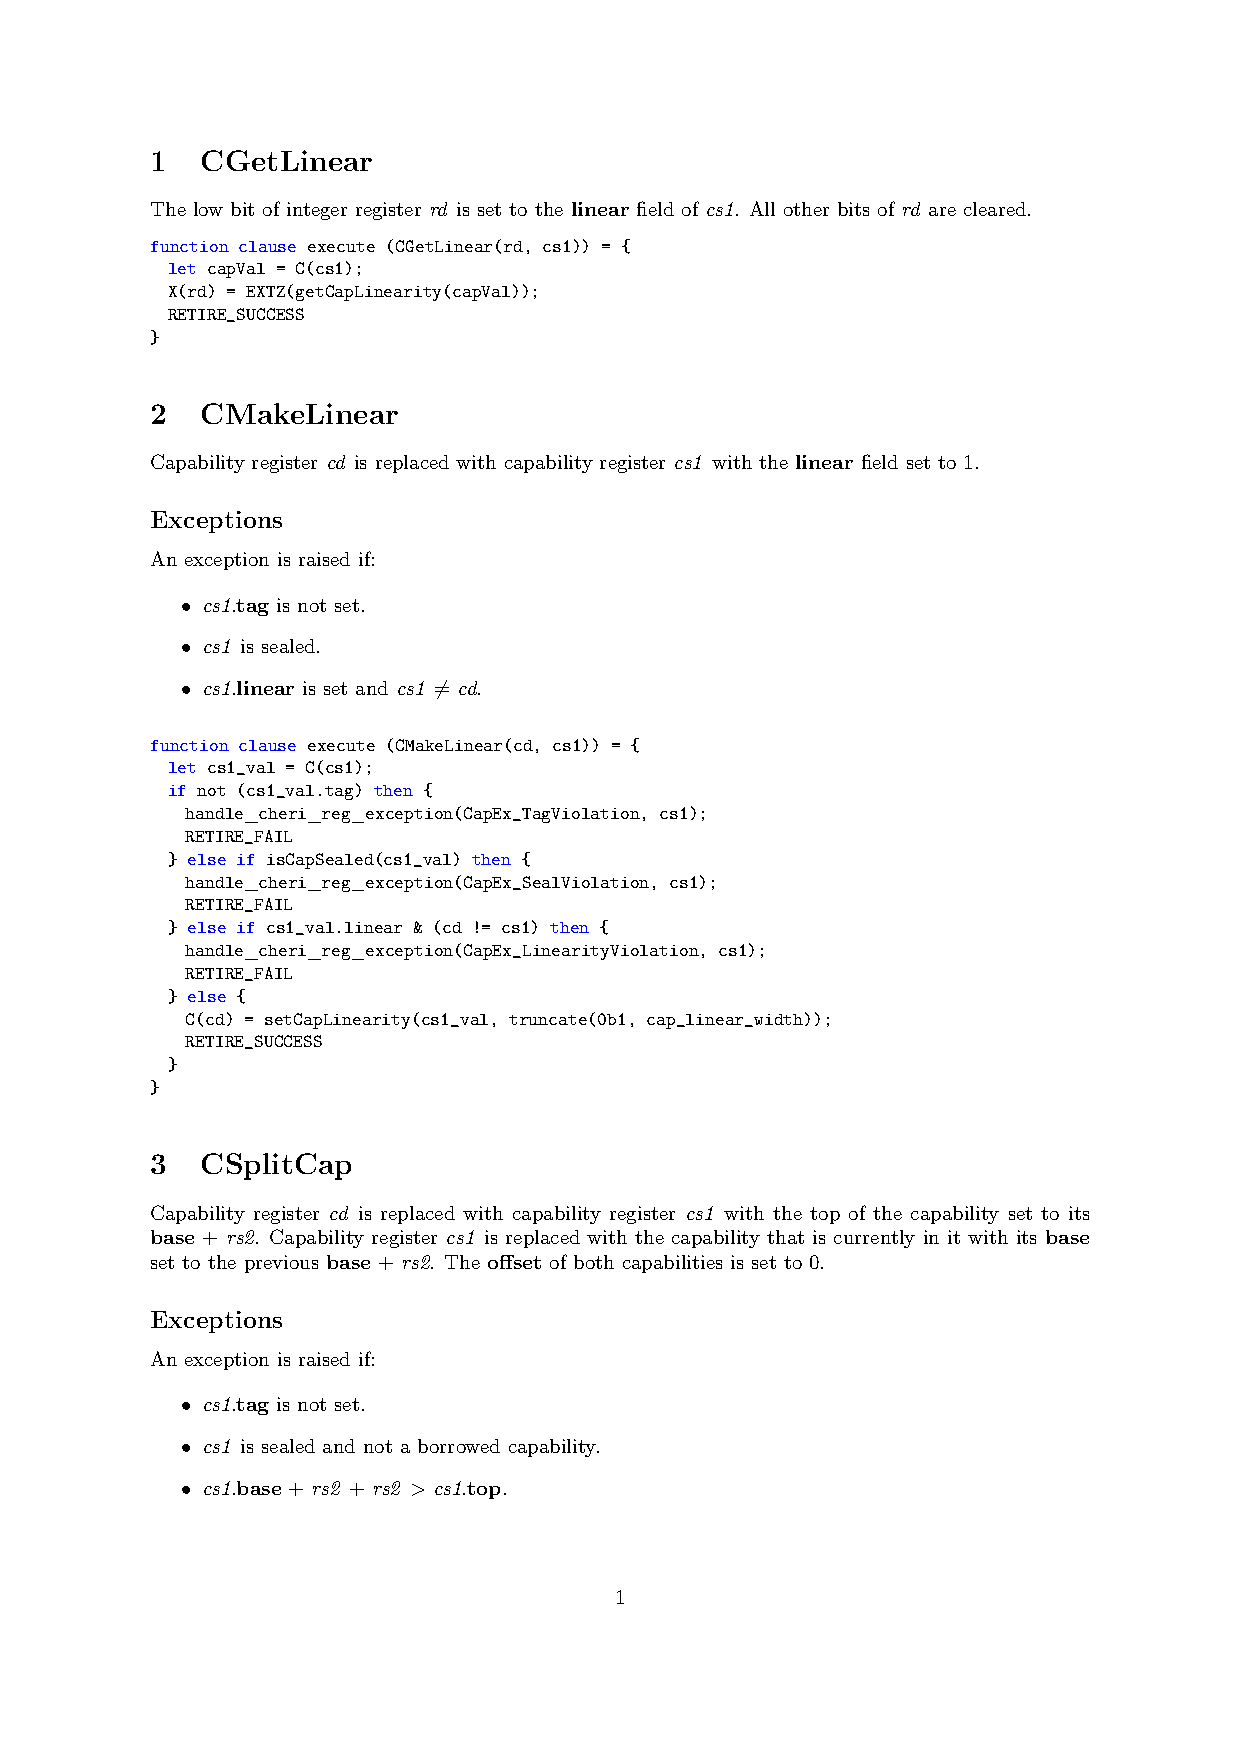
\includepdf[pages=-]{sailcode.pdf}

%%% Local Variables: 
%%% mode: latex
%%% TeX-master: "thesis"
%%% End: 

% ... and so on until
\chapter{The Last Appendix}
\label{app:n}
Appendices are numbered with letters, but the sections and subsections use
arabic numerals, as can be seen below.

\section{Lorem 20-24}
\lipsum[20-24]

\section{Lorem 25-27}
\lipsum[25-27]

%%% Local Variables: 
%%% mode: latex
%%% TeX-master: "thesis"
%%% End: 


\backmatter
% The bibliography comes after the appendices.
% You can replace the standard "abbrv" bibliography style by another one.
\bibliographystyle{abbrv}
\bibliography{references}

\end{document}

%%% Local Variables: 
%%% mode: latex
%%% TeX-master: t
%%% End: 
